\subsection{Genarazione Procedurale}
\label{ssec:generazioneproc}
Si è realizzato un ambiente virtuale 2D atto a ricostruire
la pianta di un edificio (uffici, capannoni, aule), allo scopo è stata usata una
generazione procedurale.
Il vantaggio più evidente dei livelli generati proceduralmente è la loro varietà
che portano ad ogni esecuzione, un ambiente diverso dal precedente.
Ciò significa che i robot non possono apprendere le posizioni di oggetti e
questo permette di testare l'affidabilità in casi sempre differenti.
Un altro vantaggio comune a tutte le implementazioni della generazione
procedurale è il tempo che si risparmia nello sviluppo.
%Nel nostro progetto, avremo un numero infinito di livelli unici. Se stessimo
%creando i nostri livelli manualmente, ciò sarebbe semplicemente impossibile.
%Saremmo limitati a forse una decina di livelli al massimo.
%L'utilizzo di una generazione procedurale come questa elimina questo carico di
%lavoro agli sviluppatori, aumenta la portata di ciò che è possibile.
Tra gli svantaggi, si ricorda, che la generazione procedurale di per sé non è
in alcun modo casuale.
L'assenza di controllo è una mancanza comune della generazione procedurale in
generale.
Dato che, di solito gli ambienti sono realizzati a mano da designer, lasciare
questo lavoro a un algoritmo si traduce in una significativa perdita di
controllo.
Un'altra considerazione da fare è la potenza di calcolo richiesta, nel nostro
caso, si ha solo una matrice 2D di piccole dimensioni che deve essere generata.
Tuttavia, mappe di più larga scala, avranno un costo computazionale che diventa
più significativo e deve essere preso in
considerazione.\cite{green2016procedural}

\begin{figure}[!htb]
	\centering
	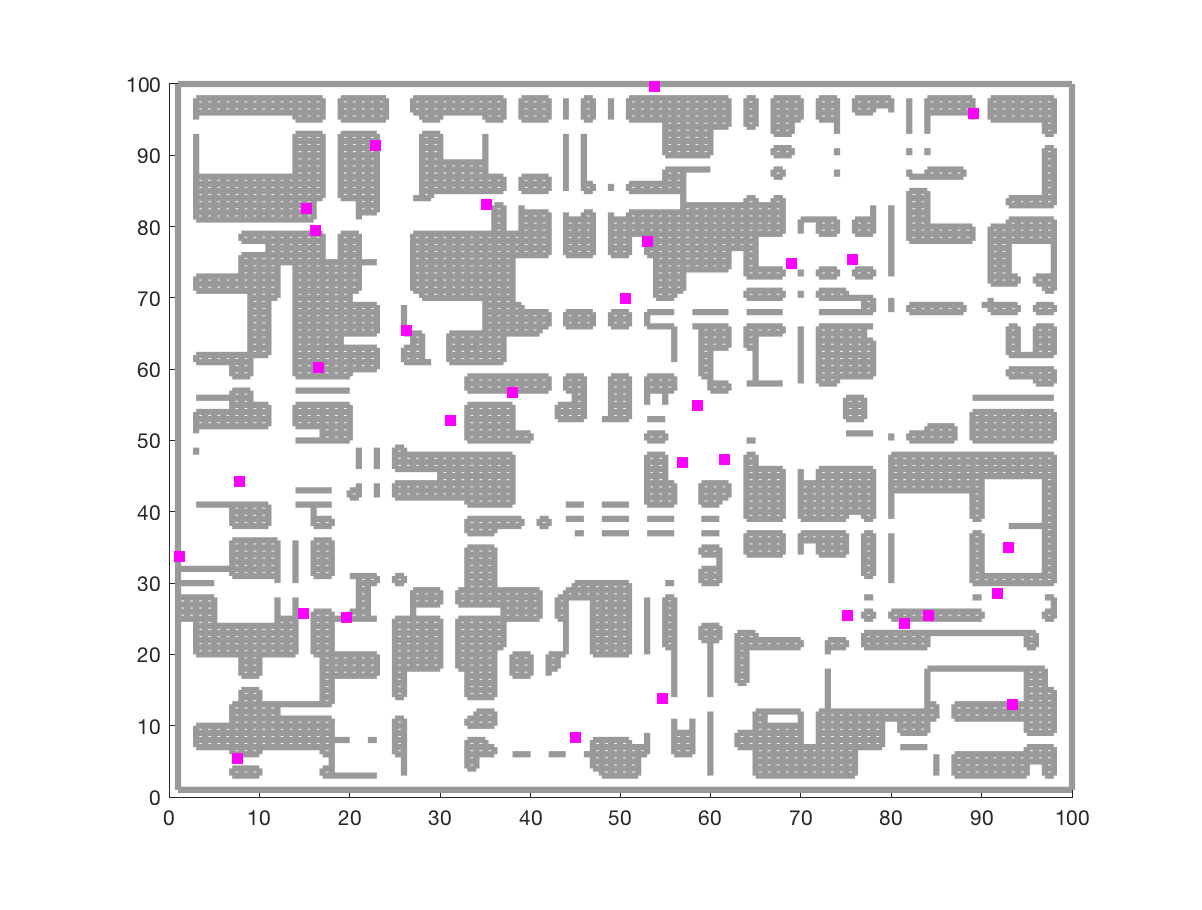
\includegraphics[width=\linewidth]{dungeon}
	\caption{esempio di scenario procedurale $100\times100$}
 	\label{fig:dungeon}
\end{figure}

\subsubsection{Binary Space Partitioning}
\label{sssec:binaryspace}
Il partizionamento dello spazio binario è un processo generico di divisione
ricorsiva di una scena in due finché il partizionamento soddisfa uno o più
requisiti.
Può essere visto come una generalizzazione di altre strutture ad albero spaziale,
uno in cui gli iperpiani che suddividono lo spazio possono avere qualsiasi
orientamento, piuttosto che essere allineati con gli assi delle coordinate.\cite{wiki:bsp}
L'albero \textbf{\emph{k-d}} è un albero binario in cui ogni nodo è un punto
k-dimensionale. Ogni nodo non foglia può essere pensato come generatore
implicito di un iperpiano scisso che divide lo spazio in due parti, note come
semispazi. I punti a sinistra di questo iperpiano sono rappresentati dal
sotto-albero sinistro di quel nodo e i punti a destra dell'iperpiano sono
rappresentati dal sotto-albero destro, come in figura \ref{fig:albero}.
La direzione dell'iperpiano viene scelta nel modo seguente: ogni nodo
dell'albero è associato a una delle dimensioni \emph{k}, con l'iperpiano
perpendicolare all'asse di quella dimensione.\cite{wiki:kdtree}

\begin{figure}[!htb]
  \centering
  \resizebox{0.7\linewidth}{!}{\begin{tikzpicture}
\draw (0,0) rectangle (10,10);
\draw [red](2,0) -- (2,4);
\draw [blue](0,4) -- (7,4);
\draw [red](4,4) -- (4,10);
\draw [red](8,0) -- (8,6);
\draw [blue](7,6) -- (10,6);
\draw [red](7,0) -- (7,10);
%add points
\foreach \Point in {(2,3),(5,4),(9,6),(4,7),(8,1),(7,2)}{
    \node at \Point {\textbullet};
};   
\end{tikzpicture}

}
  \caption{decomposizione per il set di punti.}
  \label{fig:decomposizione}
\end{figure}

\begin{figure}[!htb]
\centering
    \resizebox{0.7\linewidth}{!}{\begin{tikzpicture}
[every node/.style={fill,draw=orange,fill=orange!75,text=white,drop shadow},
accepting/.style ={green!50!black,text=white},
level distance=10mm,
level 1/.style={sibling distance=20mm},
level 2/.style={sibling distance=10mm},
level 3/.style={sibling distance=5mm}]

%k-d tree decomposition for the point set
\node (Root) {\tiny $(7,2)$}
    child { node {\tiny $(5,4)$}
    		child { node {\tiny $(2,3)$}} %3rdlevel
    			%child { node {\tiny $(1,10)$}}}%last level
    		child { node {\tiny $(4,7)$}} %3rd level
    			%child { node {\tiny $(50,50)$}}}%last level
    			}		
	child { node {\tiny $(9,6)$}
    			child { node {\tiny $(8,1)$}}
    			child [missing]{}
    		};
\end{tikzpicture}
}
\caption{risultato dell'albero \emph{k-d}.}
\label{fig:albero}
\end{figure}
